\documentclass[12pt]{jarticle}
\usepackage[dvipdfmx]{graphicx}
\usepackage{url}
\usepackage{listings,jlisting}
\usepackage{ascmac}
\usepackage{amsmath,amssymb}

%ここからソースコードの表示に関する設定
\lstset{
  basicstyle={\ttfamily},
  identifierstyle={\small},
  commentstyle={\smallitshape},
  keywordstyle={\small\bfseries},
  ndkeywordstyle={\small},
  stringstyle={\small\ttfamily},
  frame={tb},
  breaklines=true,
  columns=[l]{fullflexible},
  numbers=left,
  xrightmargin=0zw,
  xleftmargin=3zw,
  numberstyle={\scriptsize},
  stepnumber=1,
  numbersep=1zw,
  lineskip=-0.5ex
}
%ここまでソースコードの表示に関する設定

\title{知能プログラミング演習II 課題3}
\author{グループ8\\
  29114003 青山周平\\
}
\date{2019年11月05日}

\begin{document}
\maketitle

\paragraph{提出物} rep3
\paragraph{グループ} グループ8
\paragraph{メンバー}
\begin{tabular}{|c|c|c|}
  \hline
  学生番号&氏名&貢献度比率\\
  \hline\hline
  29114003&青山周平&null\\
  \hline
  29114060&後藤拓也&null\\
  \hline
  29114116&増田大輝&null\\
  \hline
  29114142&湯浅範子&null\\
  \hline
  29119016&小中祐希&null\\
  \hline
\end{tabular}



\section{課題の説明}
\begin{description}
\item[必須課題3-1] セマンティックネットのプログラムを参考に,グループメンバー全員(およびその周辺人物)についてのセマンティックネットを構築せよ.
個人レポートには自分のみ(とその周辺)に関するセマンティックネットを示し,グループレポートには全員(とその周辺)に関するセマンティックネットを示せ.
\item[必須課題3-2] フレームのプログラムを参考に,自分達の興味分野に関する知識をフレームで表現せよ.その分野の知識を表す上で必須となるスロットが何かを考え,クラスフレームを設計すること.
個人レポートには自分が作ったインスタンスフレームのみ(クラスフレームの設計担当者はクラスフレームも)を示し,グループレポートにはクラスフレームおよび全員分のインスタンスフレームを示せ.
\item[必須課題3-3] 課題3-1または3-2で作った知識表現を用いた質問応答システムを作成せよ.
なお,ユーザの質問は英語や日本語のような自然言語が望ましいが,難しければ課題2で扱ったような変数を含むパターン (クエリー) でも構わない. 
\item[発展課題3-4] 課題3-1または3-2で作った知識表現を図として示すためのユーザインターフェース(GUI) を設計し実装せよ.
\item[発展課題3-5] 上記3-3で作成した質問応答システムを,DBpediaあるいはWikidata中の知識を使って質問に答えられるよう,拡張せよ.
\end{description}

\section{必須課題3-1}
\begin{screen}
セマンティックネットのプログラムを参考に,グループメンバー全員(およびその周辺人物)についてのセマンティックネットを構築せよ.

個人レポートには自分のみ(とその周辺)に関するセマンティックネットを示し,グループレポートには全員(とその周辺)に関するセマンティックネットを示せ.
\end{screen}
私(とその周辺)に関するセマンティックネットの構造は,下図の通りである.
\begin{figure}[!hbt]
  	\begin{center}
	\end{center}
  	\caption{セマンティックネット}
\end{figure}


\section{必須課題3-2}
\begin{screen}
フレームのプログラムを参考に,自分達の興味分野に関する知識をフレームで表現せよ.その分野の知識を表す上で必須となるスロットが何かを考え,クラスフレームを設計すること.

個人レポートには自分が作ったインスタンスフレームのみ(クラスフレームの設計担当者はクラスフレームも)を示し,グループレポートにはクラスフレームおよび全員分のインスタンスフレームを示せ.
\end{screen}
私が作ったインスタンスフレームは下図のような設計となっている.
\begin{figure}[!hbt]
  	\begin{center}
  		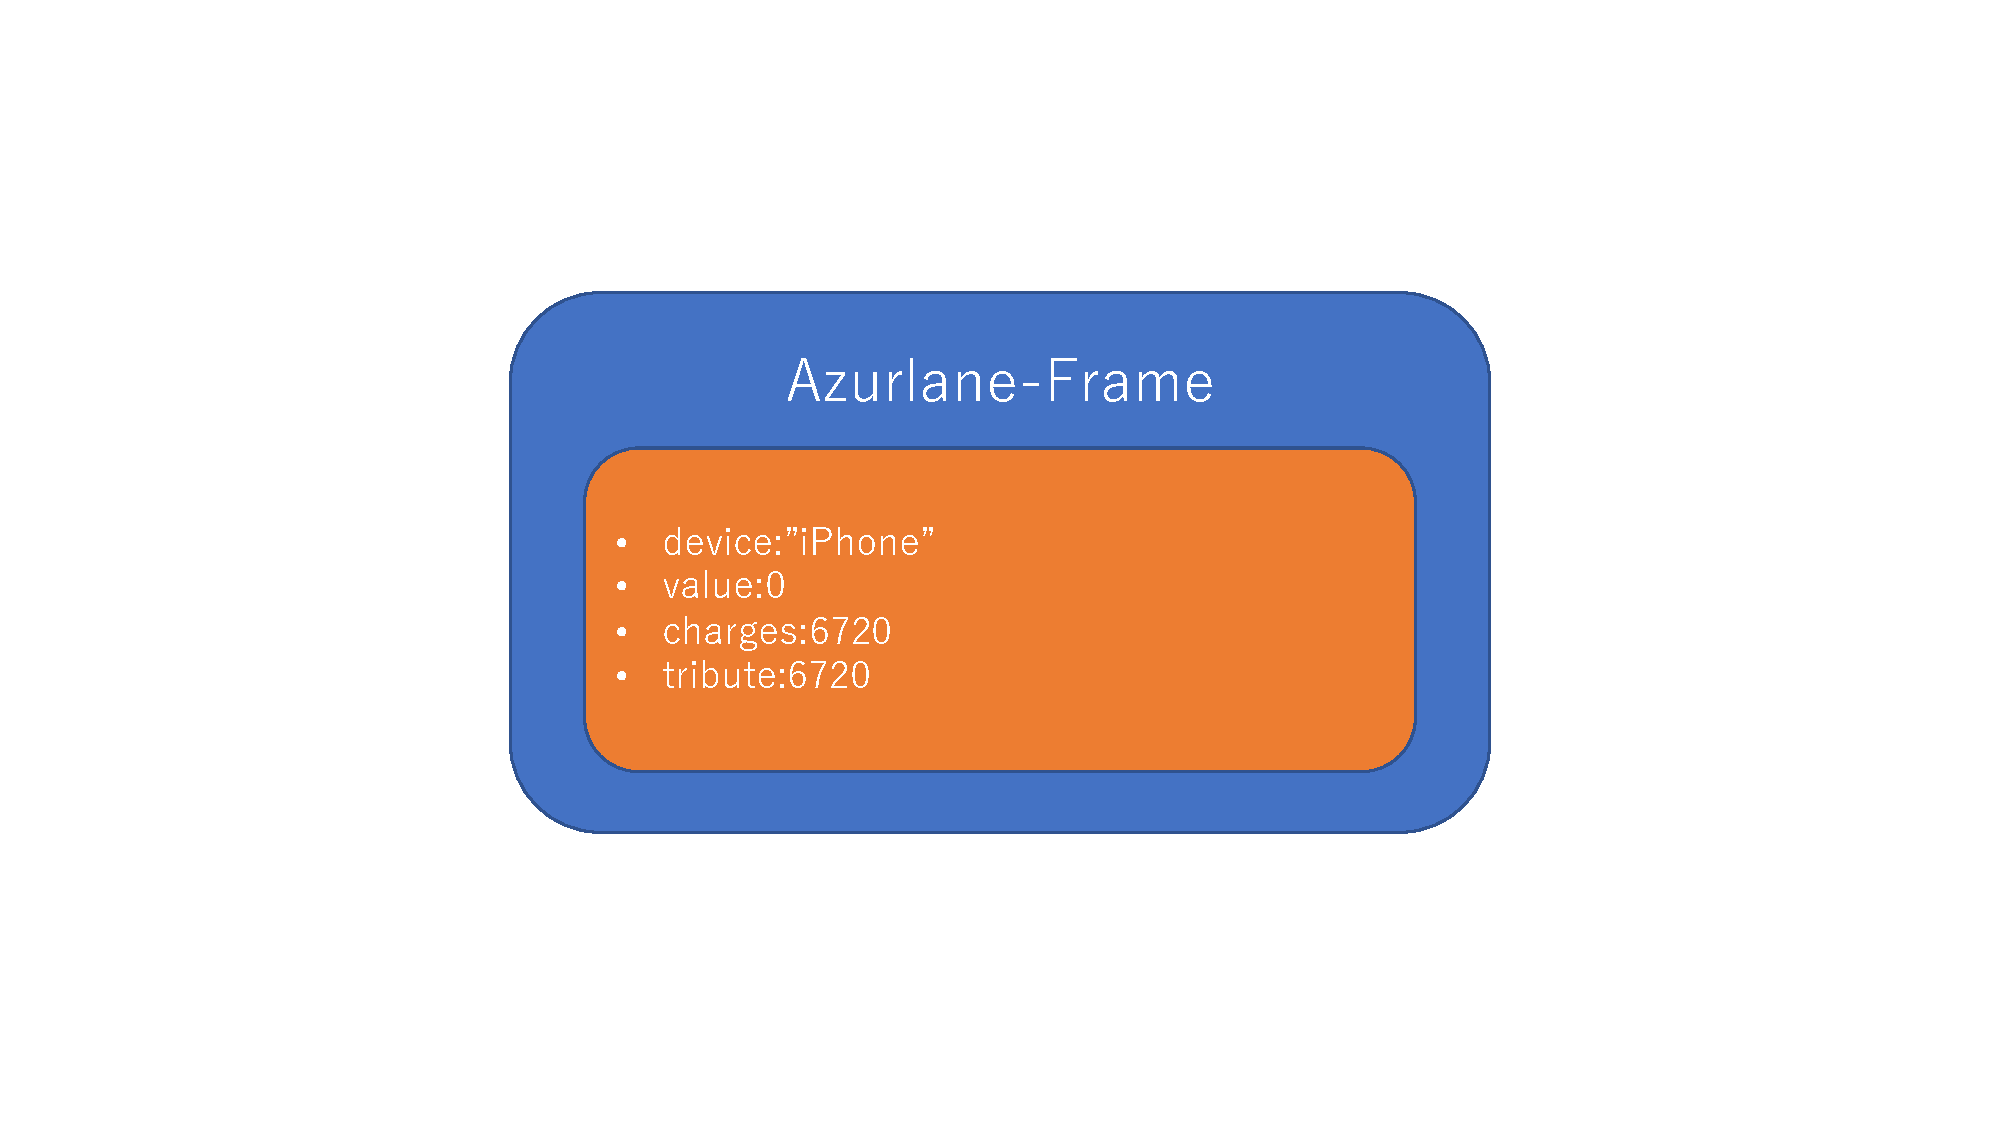
\includegraphics[scale=0.40]{images/azurlane.pdf}
	\end{center}
  	\caption{インスタンスフレーム}
\end{figure}

\clearpage

\section{発展課題3-4}
\begin{screen}
課題3-1または3-2で作った知識表現を図として示すためのユーザインターフェース(GUI) を設計し実装せよ.
\end{screen}
私の担当箇所は,発展課題3-4におけるGUIのSwingを用いた実装である.

\subsection{手法}
セマンティックネットのためのGUIを実装するにあたり,以下のような方針を立てた.
\begin{enumerate}
\item ノードやリンクのデータを受け取る.
\item ノードを表示するためのパネルを作り,リンクを表示するための描写を設定する.また,パネルをマウスで移動できるようにする.
\item 検索・追加・削除の機能を追加する.
\end{enumerate}

1.に関して,他のプログラムとのデータのやりとりの仲介プログラムを他の班員に作ってもらうことで,作業の分担・効率化を図った.

2.に関して,セマンティックネットのような複雑な図をユーザが自身で最も見やすい表示にするために,マウスによるドラッグでパネルを移動できるような仕様とした.

3.に関して,これらの機能をセマンティックネットとは別のパネルに分けたことで,より構造化された,拡張性・保守性の高い管理しやすいプログラムとなるようにした.

また,セマンティックネットのGUIを元にして,フレームのGUIも作った.

\clearpage

\subsection{実装}
セマンティックネットのGUIに関するプログラムSemNetGUI.javaには以下のクラスが含まれる.
\begin{itemize}
\item SemNetGUI: メソッドmain, クラスMenuPanelを実装した,フレームとメニューバーを実装するためのクラス.
\item RelationMap: セマンティックネット全体を管理するパネルを実装するためのクラス.
\item NodePanel: 1つのノードに関するパネルを実装するためのクラス.
\item LinkPanel: 1つのリンクに関するパネルを実装するためのクラス.
\end{itemize}

フレームのGUIに関するプログラムFrameGUI.javaには以下のクラスが含まれる.
\begin{itemize}
\item FrameGUI: メソッドmainを実装したフレームを実装するためのクラス.
\item FrameMap: 全フレームを管理するパネルを実装するためのクラス.
\item FramePanel: 1つのフレームに関するパネルを実装するための抽象クラス.
\item ClassFramePanel: クラスフレームのときに用いるFramePanelクラスを継承したクラス.
\item InstanceFramePanel: インスタンスフレームのときに用いるFramePanelクラスを継承したクラス.
\item LinkPanel: 2つのフレーム間の1つの継承関係に関するパネルを実装するためのクラス.
\end{itemize}

\subsubsection{ノードやリンクのデータを受け取る}
ノードやリンクの作成や取得にはSemanticNet.javaを呼び出す必要がある.そこで,その仲介のためのプログラムAccessData.javaを他の班員に作ってもらった.私の担当箇所であるSemNetGUI.javaからはAccessData.javaを介することでSemanticNet.javaで必要な処理をより簡単に行えるようにした.

RelationMapクラスのコンストラクタにおけるAccessDataを用いた処理を
ソースコード\ref{ad}に示す.

\begin{lstlisting}[caption=RelationMapクラスのコンストラクタ, label=ad]
    RelationMap(String filename) {
        sn = new SemanticNet();
        ad = new AccessData(sn);
        ad.start(filename);  // セマンティックネットの構築
        ...
        nodes = new HashMap<>();
        ArrayList<Node> nodeList = ad.getNodes();  // セマンティックネットからノードの取得
        ...
        links = new HashMap<>();
        ArrayList<Link> linkList = ad.getLinks();  // セマンティックネットからリンクの取得
        ...
        }
    }
\end{lstlisting}

\subsubsection{ノードを表示するためのパネルを作り,リンクを表示するための描写を設定する.また,パネルをマウスで移動できるようにする}
ノードのパネルの作成にはJPanelクラスを継承したNodePanelクラスを実装し,利用した.このパネルはマウスでドラッグできるようにする必要があるため,それを実装するためにMouseAdapterクラスのmousePressedメソッドとMouseMotionAdapterクラスのmouseDraggedメソッドをオーバライドすることで,実装した.

また,これらのイベントモデルは全て匿名クラスで実装した.これにより,ソースコードがスッキリし,挙動も分かりやすくすることができた.

NodePanelクラスのコンストラクタにおけるドラック処理を
ソースコード\ref{drag}に示す.

\begin{lstlisting}[caption=NodePanelクラスのコンストラクタ, label=drag]
    NodePanel(Node node) {
        ...
        addMouseListener(new MouseAdapter() {
            @Override
            public void mousePressed(MouseEvent e) {
                draggedAtX = e.getX();
                draggedAtY = e.getY();
            }
        });

        addMouseMotionListener(new MouseMotionAdapter() {
            @Override
            public void mouseDragged(MouseEvent e) {
                setLocation(e.getX() - draggedAtX + getLocation().x, e.getY() - draggedAtY + getLocation().y);

                for (LinkPanel lp : departFromMeLinks) {
                    lp.update();
                    lp.repaint();
                }
                for (LinkPanel lp : arriveAtMeLinks) {
                    lp.update();
                    lp.repaint();
                }
            }
        });
        ...
    }
\end{lstlisting}

まず,mousePressedメソッドではe.getX(), e.getY()メソッドによって,マウスがクリックされた時点での座標が取得される.これをNodePanelクラスのフィールドであるint型変数draggedAtX,  draggedAtYに代入し,保持している.

次にmouseDraggedメソッドでは,マウスがクリックされたままドラッグされる度にsetLocationメソッドによって自身のインスタンスの座標を更新している.ここでsetLocationにて行われている計算式について,x軸について特筆して述べる.getLocation().xはNodePanelが配置されるコンポーネントにおける座標であるのに対して,e.getX()とdraggedAtXはNodePanel内における座標である.すなわちsetLocationメソッドが実行される度にe.getX()の座標はdraggedAtXに一致するため,この計算式で正しく動作することが証明できる.

また,mouseDraggedメソッドでは,updateメソッドとrepaintメソッドの呼び出しが行われている.これにより,ノードに対応するリンクについてもパネルが更新されている. \\

リンクのパネルについて,ノードのパネルと違い,パネルの移動だけでなく,パネルの拡大縮小・矢印の再描写が求められる.そこで,パネルの座標と大きさの設定を行えるsetSizeメソッド,setSizeメソッドを用いて更にラベルの位置も更新するupdateメソッドを実装した.
LinkPanelクラス内のこれらのメソッドを
ソースコード\ref{update}に示す.

\begin{lstlisting}[caption=setSizeメソッド・updateメソッド, label=update]
    void setSize() {
        int lpX = getLeft();
        int lpY = getTop();
        int lpWidth = getRight() - lpX;
        int lpHeight = getBtm() - lpY;
        setBounds(lpX, lpY, lpWidth, lpHeight);
    }

    void update() {
        Rectangle source = tail.getBounds();
        Rectangle distance = head.getBounds();
        setShortestDistance(source, distance);
        setSize();

        int fitX = -(mainPanel.getWidth() / 2);
        int fitY = -(mainPanel.getHeight() / 2);
        mainPanel.setLocation((getRight() - getLeft()) / 2 + fitX, (getBtm() - getTop()) / 2 + fitY);
    }
\end{lstlisting}

getLeft, getTop, getRight, getBtmメソッドはパネルの座標を取得するために実装されている.

\subsubsection{検索・追加・削除の機能を追加する}
内部クラス

\subsubsection{セマンティックネットのGUIを元にして,フレームのGUIを作る}
FrameGUI.javaは,基本的にSemNetGUI.javaを元にして作られている.しかしFrameにはNodeと異なり,クラスフレームやインスタンスフレームといった概念が存在する.これを解決するために,FramePanelクラスを抽象クラスとして,クラスフレームのためのパネルにはClassFramePanelクラス,インスタンスフレームのためのパネルにはInstanceFramePanelクラスを実装して利用することで,それぞれの挙動に合わせたパネルを作り分けることができた.

ClassFramePanelクラス,InstanceFramePanelクラスを
ソースコード\ref{frame}に示す.

\begin{lstlisting}[caption=ClassFramePanelクラス・InstanceFramePanelクラス, label=frame]
class ClassFramePanel extends FramePanel {
    private ArrayList<InstanceFramePanel> list;

    ClassFramePanel(String name, List<String> slotLabels, List<String> values) {
        super(name, slotLabels, values);
        list = new ArrayList<>();
    }

    void addInstance(InstanceFramePanel ifp) {
        list.add(ifp);
    }
}

class InstanceFramePanel extends FramePanel {
    private ClassFramePanel par;

    InstanceFramePanel(String name, ClassFramePanel cfp, List<String> values) {
        super(name, new ArrayList(cfp.getSlots().keySet()), values);
        par = cfp;
        cfp.addInstance(this);
    }
}
\end{lstlisting}

\clearpage

\subsection{実行例}
UnifyGUIを実行したところ,下図のような画面が得られる.

\begin{figure}[!hbt]
  	\begin{center}
	\end{center}
  	\caption{初期状態}
\end{figure}
\clearpage


\subsection{考察}


\section{感想}


% 参考文献
\begin{thebibliography}{99}
TATSUO IKURA: 『Swingを使ってみよう - Java GUIプログラミング』 https://www.javadrive.jp/tutorial/ (2019/11/05アクセス) \\
\end{thebibliography}

\end{document}
